% Options for packages loaded elsewhere
\PassOptionsToPackage{unicode}{hyperref}
\PassOptionsToPackage{hyphens}{url}
\PassOptionsToPackage{dvipsnames,svgnames,x11names}{xcolor}
%
\documentclass[
  10pt,
  letterpaper,
  DIV=11,
  numbers=noendperiod]{scrartcl}

\usepackage{amsmath,amssymb}
\usepackage{iftex}
\ifPDFTeX
  \usepackage[T1]{fontenc}
  \usepackage[utf8]{inputenc}
  \usepackage{textcomp} % provide euro and other symbols
\else % if luatex or xetex
  \usepackage{unicode-math}
  \defaultfontfeatures{Scale=MatchLowercase}
  \defaultfontfeatures[\rmfamily]{Ligatures=TeX,Scale=1}
\fi
\usepackage{lmodern}
\ifPDFTeX\else  
    % xetex/luatex font selection
    \setmainfont[]{Helvetica}
    \setmonofont[]{Roboto}
\fi
% Use upquote if available, for straight quotes in verbatim environments
\IfFileExists{upquote.sty}{\usepackage{upquote}}{}
\IfFileExists{microtype.sty}{% use microtype if available
  \usepackage[]{microtype}
  \UseMicrotypeSet[protrusion]{basicmath} % disable protrusion for tt fonts
}{}
\makeatletter
\@ifundefined{KOMAClassName}{% if non-KOMA class
  \IfFileExists{parskip.sty}{%
    \usepackage{parskip}
  }{% else
    \setlength{\parindent}{0pt}
    \setlength{\parskip}{6pt plus 2pt minus 1pt}}
}{% if KOMA class
  \KOMAoptions{parskip=half}}
\makeatother
\usepackage{xcolor}
\setlength{\emergencystretch}{3em} % prevent overfull lines
\setcounter{secnumdepth}{2}
% Make \paragraph and \subparagraph free-standing
\makeatletter
\ifx\paragraph\undefined\else
  \let\oldparagraph\paragraph
  \renewcommand{\paragraph}{
    \@ifstar
      \xxxParagraphStar
      \xxxParagraphNoStar
  }
  \newcommand{\xxxParagraphStar}[1]{\oldparagraph*{#1}\mbox{}}
  \newcommand{\xxxParagraphNoStar}[1]{\oldparagraph{#1}\mbox{}}
\fi
\ifx\subparagraph\undefined\else
  \let\oldsubparagraph\subparagraph
  \renewcommand{\subparagraph}{
    \@ifstar
      \xxxSubParagraphStar
      \xxxSubParagraphNoStar
  }
  \newcommand{\xxxSubParagraphStar}[1]{\oldsubparagraph*{#1}\mbox{}}
  \newcommand{\xxxSubParagraphNoStar}[1]{\oldsubparagraph{#1}\mbox{}}
\fi
\makeatother


\providecommand{\tightlist}{%
  \setlength{\itemsep}{0pt}\setlength{\parskip}{0pt}}\usepackage{longtable,booktabs,array}
\usepackage{calc} % for calculating minipage widths
% Correct order of tables after \paragraph or \subparagraph
\usepackage{etoolbox}
\makeatletter
\patchcmd\longtable{\par}{\if@noskipsec\mbox{}\fi\par}{}{}
\makeatother
% Allow footnotes in longtable head/foot
\IfFileExists{footnotehyper.sty}{\usepackage{footnotehyper}}{\usepackage{footnote}}
\makesavenoteenv{longtable}
\usepackage{graphicx}
\makeatletter
\def\maxwidth{\ifdim\Gin@nat@width>\linewidth\linewidth\else\Gin@nat@width\fi}
\def\maxheight{\ifdim\Gin@nat@height>\textheight\textheight\else\Gin@nat@height\fi}
\makeatother
% Scale images if necessary, so that they will not overflow the page
% margins by default, and it is still possible to overwrite the defaults
% using explicit options in \includegraphics[width, height, ...]{}
\setkeys{Gin}{width=\maxwidth,height=\maxheight,keepaspectratio}
% Set default figure placement to htbp
\makeatletter
\def\fps@figure{htbp}
\makeatother
% definitions for citeproc citations
\NewDocumentCommand\citeproctext{}{}
\NewDocumentCommand\citeproc{mm}{%
  \begingroup\def\citeproctext{#2}\cite{#1}\endgroup}
\makeatletter
 % allow citations to break across lines
 \let\@cite@ofmt\@firstofone
 % avoid brackets around text for \cite:
 \def\@biblabel#1{}
 \def\@cite#1#2{{#1\if@tempswa , #2\fi}}
\makeatother
\newlength{\cslhangindent}
\setlength{\cslhangindent}{1.5em}
\newlength{\csllabelwidth}
\setlength{\csllabelwidth}{3em}
\newenvironment{CSLReferences}[2] % #1 hanging-indent, #2 entry-spacing
 {\begin{list}{}{%
  \setlength{\itemindent}{0pt}
  \setlength{\leftmargin}{0pt}
  \setlength{\parsep}{0pt}
  % turn on hanging indent if param 1 is 1
  \ifodd #1
   \setlength{\leftmargin}{\cslhangindent}
   \setlength{\itemindent}{-1\cslhangindent}
  \fi
  % set entry spacing
  \setlength{\itemsep}{#2\baselineskip}}}
 {\end{list}}
\usepackage{calc}
\newcommand{\CSLBlock}[1]{\hfill\break\parbox[t]{\linewidth}{\strut\ignorespaces#1\strut}}
\newcommand{\CSLLeftMargin}[1]{\parbox[t]{\csllabelwidth}{\strut#1\strut}}
\newcommand{\CSLRightInline}[1]{\parbox[t]{\linewidth - \csllabelwidth}{\strut#1\strut}}
\newcommand{\CSLIndent}[1]{\hspace{\cslhangindent}#1}

\KOMAoption{captions}{tableheading}
\usepackage[dvipsnames]{xcolor} % colors
\newcommand{\ear}[1]{{\textcolor{blue}{#1}}}
\newcommand{\svp}[1]{{\textcolor{RedOrange}{#1}}}
\newcommand{\hh}[1]{{\textcolor{Green}{#1}}}
\makeatletter
\@ifpackageloaded{caption}{}{\usepackage{caption}}
\AtBeginDocument{%
\ifdefined\contentsname
  \renewcommand*\contentsname{Table of contents}
\else
  \newcommand\contentsname{Table of contents}
\fi
\ifdefined\listfigurename
  \renewcommand*\listfigurename{List of Figures}
\else
  \newcommand\listfigurename{List of Figures}
\fi
\ifdefined\listtablename
  \renewcommand*\listtablename{List of Tables}
\else
  \newcommand\listtablename{List of Tables}
\fi
\ifdefined\figurename
  \renewcommand*\figurename{Figure}
\else
  \newcommand\figurename{Figure}
\fi
\ifdefined\tablename
  \renewcommand*\tablename{Table}
\else
  \newcommand\tablename{Table}
\fi
}
\@ifpackageloaded{float}{}{\usepackage{float}}
\floatstyle{ruled}
\@ifundefined{c@chapter}{\newfloat{codelisting}{h}{lop}}{\newfloat{codelisting}{h}{lop}[chapter]}
\floatname{codelisting}{Listing}
\newcommand*\listoflistings{\listof{codelisting}{List of Listings}}
\makeatother
\makeatletter
\makeatother
\makeatletter
\@ifpackageloaded{caption}{}{\usepackage{caption}}
\@ifpackageloaded{subcaption}{}{\usepackage{subcaption}}
\makeatother

\ifLuaTeX
  \usepackage{selnolig}  % disable illegal ligatures
\fi
\usepackage{bookmark}

\IfFileExists{xurl.sty}{\usepackage{xurl}}{} % add URL line breaks if available
\urlstyle{same} % disable monospaced font for URLs
\hypersetup{
  pdftitle={A Guide to Designing Experiments to Test Statistical Graphics},
  pdfauthor={Emily Robinson; Heike Hofmann; Susan Vanderplas},
  colorlinks=true,
  linkcolor={blue},
  filecolor={Maroon},
  citecolor={Blue},
  urlcolor={Blue},
  pdfcreator={LaTeX via pandoc}}


\title{A Guide to Designing Experiments to Test Statistical Graphics}
\author{Emily Robinson \and Heike Hofmann \and Susan Vanderplas}
\date{2024-11-01}

\begin{document}
\maketitle
\begin{abstract}
In this paper, we discuss considerations and methods for experimentally
testing visualizations. We discuss levels of user engagement with
graphics, common issues when developing a sampling or data generation
model, the importance of pilot testing, and data analysis methods. Along
the way, we also provide recommendations of how to avoid some of the
unique pitfalls of human testing in statistical and visualization
research.
\end{abstract}


\section{Introduction}\label{introduction}

Charts and data visualizations are primary methods of communicating
scientific information to the public in what creators hope is an
easy-to-digest, visually attractive form. There are many strategies for
creating charts and graphs, from Tufte-esque minimalism (Tufte, 1991) to
charts designed with extra imagery and aesthetic appeal that draw the
viewer's attention and persist in memory (Cairo, 2012). For a specific
type of data, there are also usually many different chart forms to
display that data: for instance, if we have a set of categorical data
and we wish to show the relative proportions of each category, we could
do so using a stacked bar chart or the polar equivalent, a pie chart.
There have been several attempts to list out all of the types of charts
(Ribecca, 2022), create a taxonomy of charts (Bertin \& Berg, 1983;
Desnoyers, 2011), and even to classify charts using a domain-specific
grammar of graphics (Wilkinson, 1999). With all of the different design
choices available, how are chart creators to know what is the best
approach for communicating data to the appropriate audience?

While there are heuristics, rules-of-thumb, and various guidelines
(Allen \& Erhardt, 2016; Few, 2006; Haemer, 1948; {``Joint Committee on
Standards for Graphic Presentation,''} 1915; Kosslyn, 2006) for creating
useful and visually attractive charts, the best way to establish the
efficacy of various design decisions is to test charts: evaluate them
under controlled conditions, and gather appropriate data (Cleveland et
al., 1988; Cleveland \& McGill, 1985) to compare different
representations of the same data. It is extremely challenging to design
studies which strike the right combination of internal and external
validity. Simply asking people to read quantities off of a graph may not
generalize beyond the questions asked or the data used in the chart
(Croxton, 1932; Croxton \& Stryker, 1927; Eells, 1926; Huhn, 1927), but
designing a study that is sufficiently robust to those issues requires
manipulation of so many factors as to be functionally close to
impossible to control or manipulate in a single experiment. In this
paper, we attempt to distill the experience gained from conducting
several different types of graphics experiments (Hofmann et al., 2012;
Robinson, 2022; VanderPlas et al., 2019; Vanderplas et al., 2024;
VanderPlas \& Hofmann, 2015, 2017), discussing the use of different
testing methods (Vanderplas et al., 2020), the process of designing a
graphical experiment, and analysis of the resulting empirical data. It
is our hope that this paper will lower the barriers that exist for
conducting empirical graphics research and reduce the probability of
costly mistakes.

Section~\ref{sec-testing-methods} discusses different methods for
testing graphics, and which methods best address different levels of
user engagement. In Section~\ref{sec-model-dev}, we discuss the process
of developing a data-generating model used to control the statistical
features of data in the tested visualizations. Model development is a
nuanced and iterative process that ultimately determines the success and
generalizability of the experimental results. We explore different
experimental design considerations in Section~\ref{sec-exp-design} and
then move to the importance of pilot testing in
Section~\ref{sec-pilot-test}. Finally, we provide some common analysis
strategies in Section~\ref{sec-analysis}, including strategies for
handling the unexpected data features which are so common in graphical
testing experiments.

\section{Testing Methods and User Engagement}\label{sec-testing-methods}

There are many different testing methods used to empirically assess
graphics. While it is certainly possible to use equipment such as
eye-tracking devices, this paper focuses primarily focus on studies
conducted without additional equipment, and primarily online, because
these experiments have the lowest overhead, offer relatively fast data
collection, and provide useful results, for well-designed experiments.
The toolkit used for these experiments is R-based (R Core Team, 2022),
and includes ggplot2 (Wickham, 2016) and Shiny (Chang et al., 2021) as
primary components, as well as JavaScript (including D3 (Bostock et al.,
2011)) to customize the Shiny interface for many of the experiments.
While we prefer this set of tools, most of the observations described
here apply to a wide variety of different workflows for graphical
experimentation.

One primary concern when testing graphics is the level of user
engagement required. For instance, testing whether someone can detect an
effect such as a trend line in noisy data is a \emph{perceptual}
question best addressed using methods which allow the user to interact
with the data on a basic visual level. Sometimes, it is possible to set
up a scenario where the user adjusts the plot directly, as in an
experiment testing the strength of the sine illusion experiment
(VanderPlas \& Hofmann, 2015): users adjusted the strength of the
illusion correction until the lines appeared to be the same length,
providing a direct measure of the magnitude of the sine illusion's
effect, as in Figure~\ref{fig-sine-illusion}. In other situations, it
may be possible to have the user directly interact with the plot, as in
Vanderplas et al. (2024), where participants were asked to rotate and
interact with a 3D rendered bar chart; the application then records all
relevant user interactions to provide insight into the visual
comparisons the user may have been performing as a supplement to the
explicitly provided estimates.

\begin{figure}

\centering{

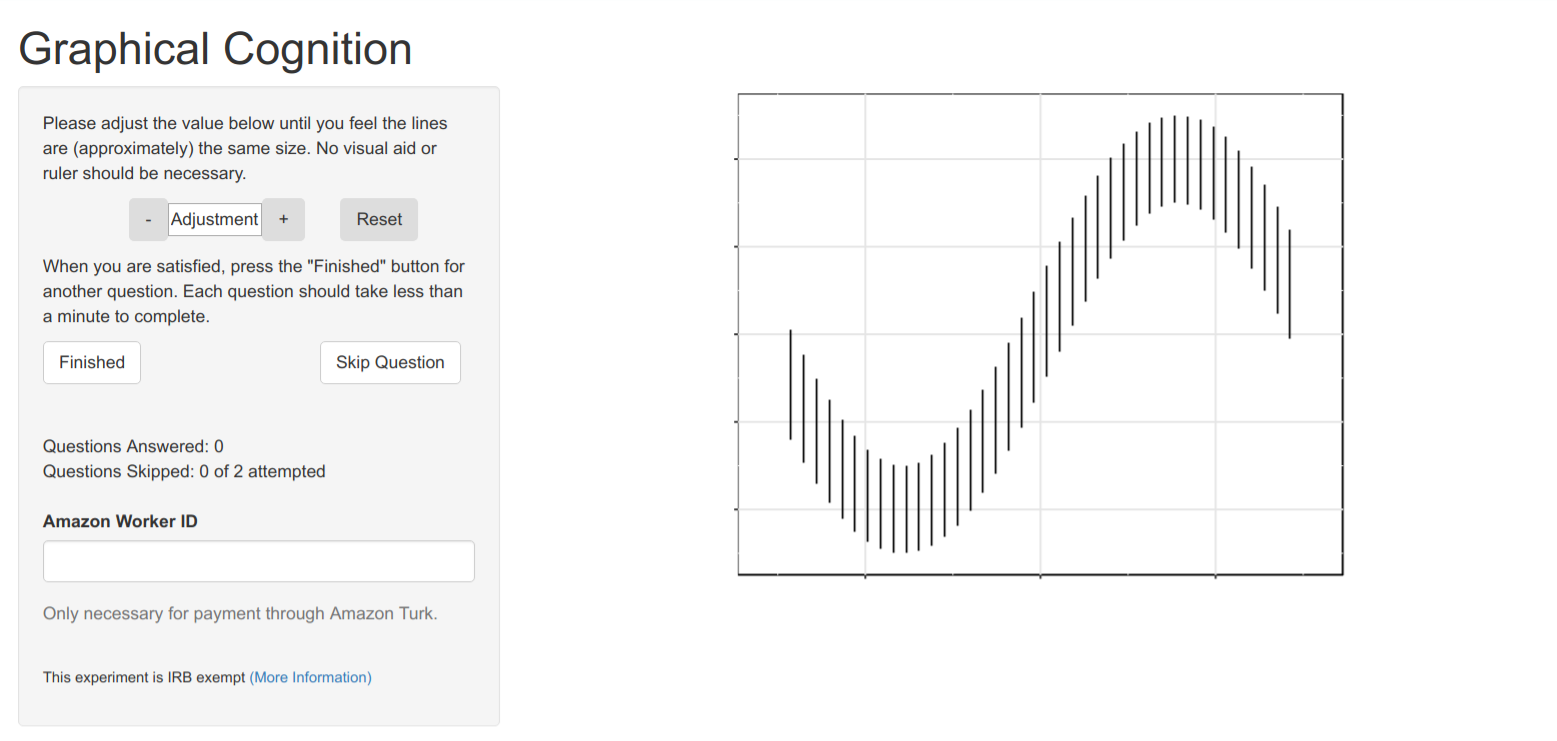
\includegraphics{sine_illusion_screenshot.png}

}

\caption{\label{fig-sine-illusion}Direct adjustment of a plot in a
perceptual task}

\end{figure}%

Statistical lineups (Buja et al., 2009; Wickham et al., 2010) are
another useful testing tool for perceptual questions such as ``which
chart displays this data more clearly'' (Hofmann et al., 2012) while
simultaneously assessing the significance of the graphical finding in
the chart. As in the criminal procedure, lineups embed a target plot
with signal into an array of 19 other innocent ``null'' plots that show
only noise. If viewers consistently pick the target plot at a higher
rate than any of the 19 null plots, the target plot is said to be
visually significant (Loy \& Hofmann, 2013; Majumder et al., 2013) and a
``see'' value (the visual analogue of a \(p\)-value for a statistical
test) can be calculated (Chowdhury et al., 2020; VanderPlas et al.,
2021). In another variation of the statistical lineup procedure, two
models are compared, with target plots from each model embedded in the
array of 20 total plots; the remaining null plots are constructed from a
mixture model that blends the two competing models. This variation
allows the experimenter to assess graphical design choices to determine
whether they effectively emphasize structural differences in the data
and assign a hierarchy of visual attributes (VanderPlas \& Hofmann,
2017). Statistical lineups do not require the experimenter to provide
any contextual information for the data: all of the necessary
information is embedded in the choice of a null statistical model, which
is convenient for testing purposes, but does not allow for testing the
viewer's understanding of the information shown in the chart.

To assess the viewer's \emph{understanding} of information shown in a
chart, we must ask questions and allow the user to provide feedback.
User feedback may be collected on a numerical scale or through the use
of written comments, recorded ``think-aloud'' processes, and other more
qualitative interaction methods. In some studies, asking users to
interpret a chart within a larger scenario can be effective, as in
Figure~\ref{fig-estimation-describe}, while in others it is more helpful
to ask users to explain answers. In lineup studies, asking users why a
specific panel was chosen can provide rich insight into otherwise
confusing numerical results. While we have not (to date) recorded users
talking out loud about what they are seeing, think aloud methods could
be implemented within a Shiny application, with audio recordings saved
to the server for transcription and analysis (Dunbar, 1995;
Kirschenbaum, 2003; Trafton et al., 2000); it is even possible that
these recordings could be automatically transcribed using text-to-speech
functions of large language models.

\begin{figure}

\centering{

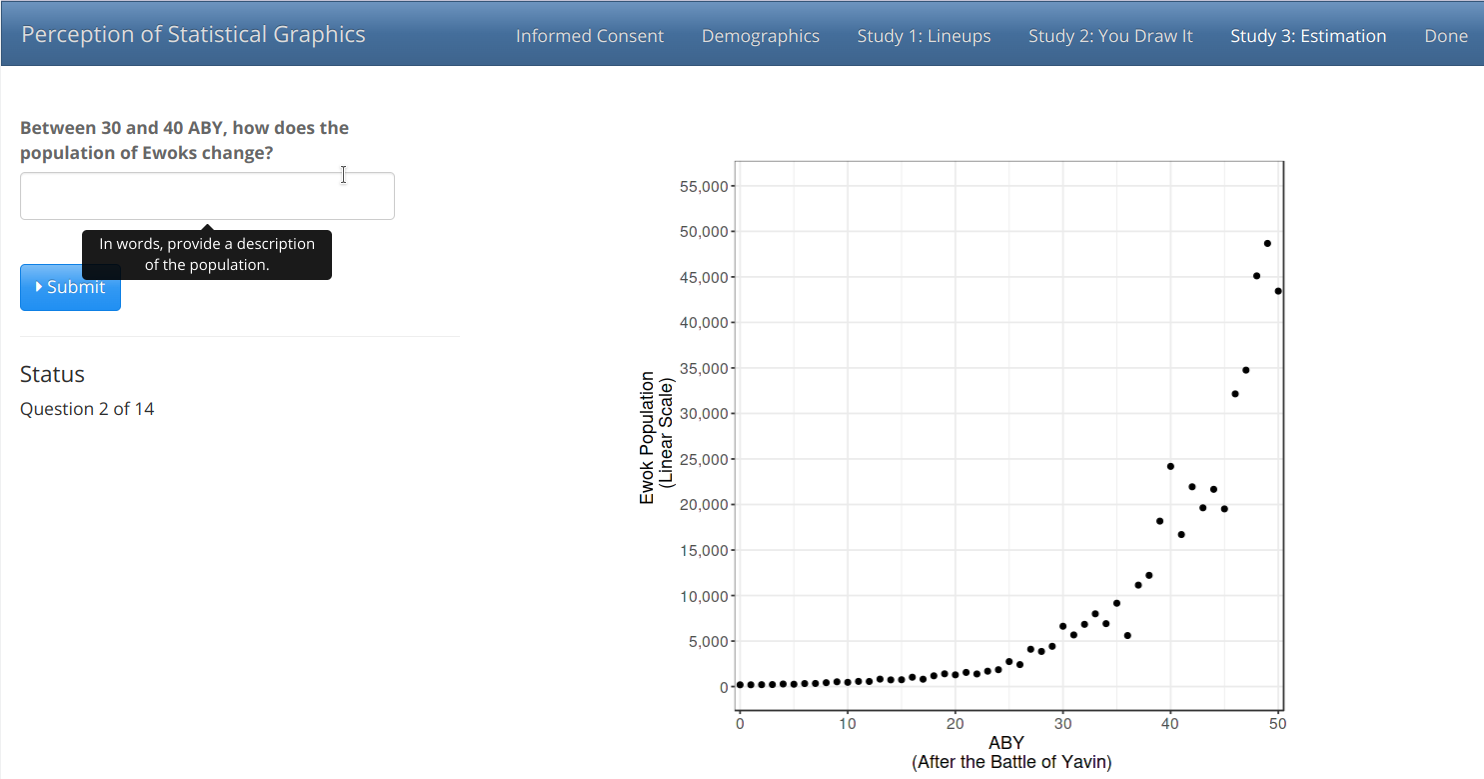
\includegraphics{Estimation_describe_plot_crop.png}

}

\caption{\label{fig-estimation-describe}This question asks users to
write out a description of how the population of Ewoks changes over
time, without any further cues, to determine whether participants
default to multiplicative or additive language descriptions.}

\end{figure}%

Of course, in an online, asynchronous experiment, every user interaction
with the testing materials (typically hosted on a web page) can also be
recorded along with time stamps, mouse positions, browser size and
screen resolution, and other information. While we have not used this
type of information heavily in our experimental analyses thus far, in
most experiments, we collect time stamp data in order to assess how long
participants spend on each question. Typically, the first round of test
questions takes the longest for participants to complete. Additional
replicates do not usually affect accuracy (i.e.~there is no immediate
learning effect) until after `too many' tests cognitive fatigue proves
to be detrimental to accuracy (Chowdhury et al., 2018). This sweet spot
between replicates and fatigue depends on the cognitive burden in each
test and should factor into designing the experiment. In some
experiments, we have provided participants with supportive tools, such
as ``scratch pads'' and calculators built into the Shiny application to
support the complex calculations required to answer higher-level
numerical estimation questions (Figure~\ref{fig-estimation-calc}). In
order to be supportive, the tools must be easy to use, but assuming this
bar is met, the tools can reduce participant cognitive load while
recording a wealth of information. This information provides real
insight into how participants were looking at the data, what strategies
they tried and discarded for reading the chart, and what visual
estimation methods were used. While systematic analysis and modeling of
this messy data may be difficult, the insights provided can be extremely
useful.

\begin{figure}

\centering{

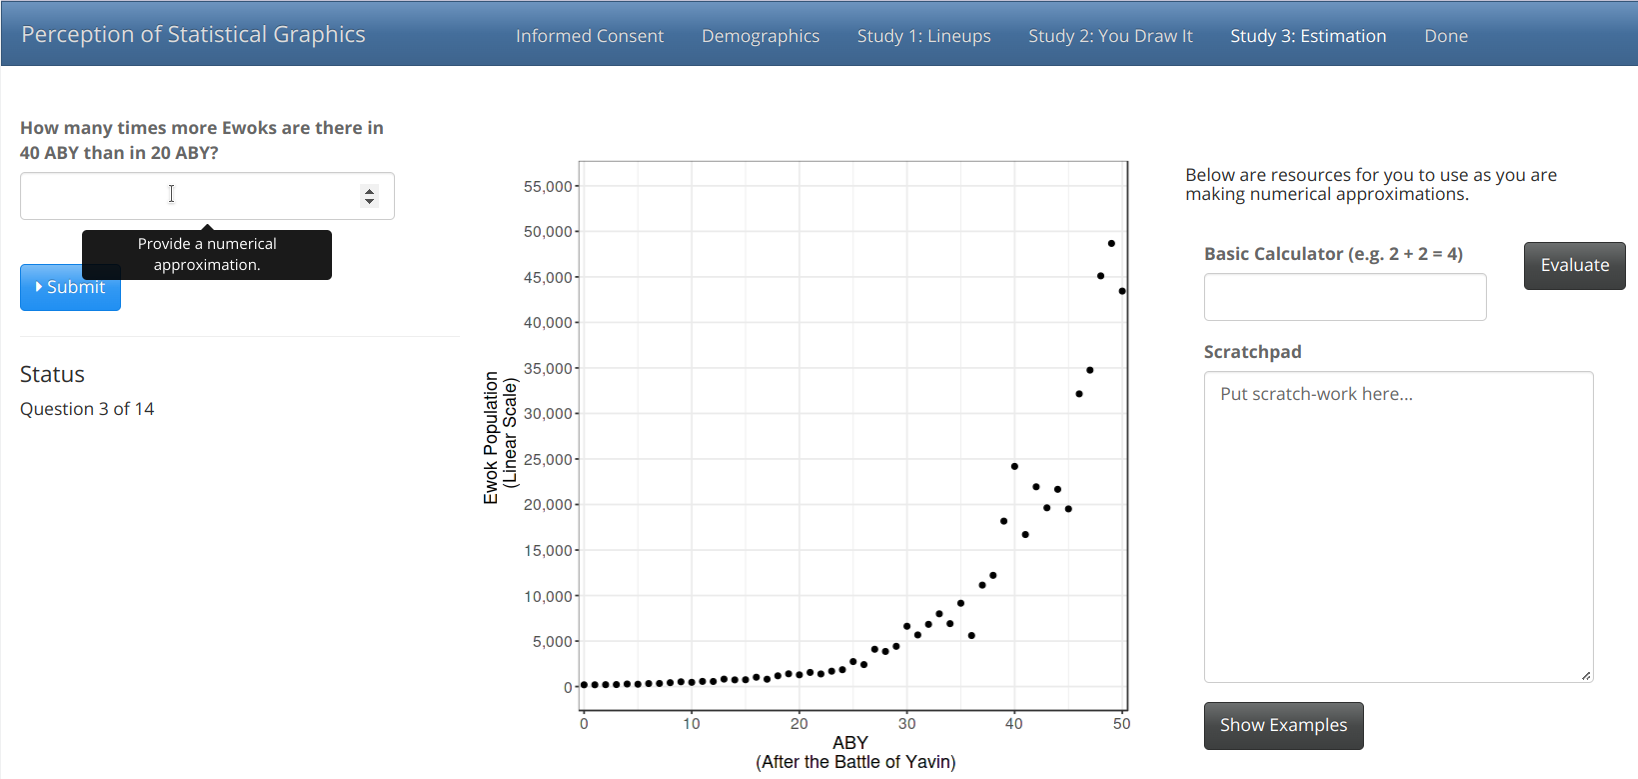
\includegraphics{Estimation_numerical_screenshot_crop.png}

}

\caption{\label{fig-estimation-calc}This question asks participants for
a numerical estimate, but provides a basic calculator and scratchpad.
All user interactions with the calculator and scratchpad are logged,
providing insight into the user's thought process and estimation
strategy.}

\end{figure}%

One of the most difficult components of designing an experiment which
asks users to directly estimate information from a chart using a full
scenario (background information, etc. as well as contextual details
from the chart) is that the questions must be extremely carefully
constructed. Mathematics education researchers provide guidelines for
selecting different levels of questioning in order to assess graph
comprehension: literal reading of the data, reading between the data,
and reading beyond the data (Curcio, 1987; Friel et al., 2001; Glazer,
2011; Wood, 1968). In a recent study, we identified questions based on
this framework to evaluate direct estimates and extend those estimates
to make comparisons between two points.

Even when great care is taken with the construction of the question,
participant answer accuracy is fundamentally limited by the fact that
many participants do not read and interpret the question with the care
and precision that it was written. Questions that ask participants to
e.g.~estimate the multiplicative change in a quantity at two time points
may be misunderstood as asking for an estimate of the additive
difference, and the resulting estimates are then one or more orders of
magnitude off of the correct answer. This is one area where lineup
methods are convenient - they do not depend on participants to
understand the nuances of language or scenarios built around the chart
under investigation. However, in some situations it may be sufficient to
ask participants to estimate direct numerical quantities that have
little contextual information, as done in (VanderPlas et al., 2019) when
assessing the accuracy of framed plots re-created from the Statistical
Atlas.

Another useful measurement strategy is to require participants to
\emph{engage directly} with an interactive visualization. This is useful
in a directed task, where users are asked to interact with the chart in
a specific way and the result is recorded, but it is also possible to
use interactive visualizations in an open-ended task, recording how
users engage with the graphic in an exploratory (as opposed to
goal-directed) manner. In one recent experiment, we asked participants
to forecast an exponential trend, with data presented on either a linear
or log scale. Using JavaScript code modified from New York Times
interactive graphics ``You Draw It'' features (Katz, 2017), we had users
draw trend lines with their computer mouse and make forecasts directly
on interactive charts, with the data and user-drawn predictions recorded
to our database. With interactive graphics rendered using JavaScript (or
other web libraries), the only limit to the types of questions one can
ask in testing graphics is one's ability to write code to interact with
the visualization library. This type of testing method can be extremely
natural for participants, but it also is hard to generalize when
discussing testing methods because of the potential range of
applications where it might be employed.

Whichever testing method is chosen should be appropriate to the type of
question under investigation and the level of visual and cognitive
engagement required to answer that question. While lineups are excellent
tools for assessing perceptual questions, they cannot address questions
aimed at understanding how people use charts within the wider context of
a story or practical task; this requires more direct methods with higher
ecological validity.

All of the testing methods described here require significant work to
develop a strategy for data generation appropriate for testing the
underlying question. For instance, when testing the perception of
exponential growth, we had to develop a model which would generate data
with varying growth rates, but where the data had a pre-specified domain
and range. The data generating model is particularly critical when using
lineups, as the null sampling model must replicate the important visual
features in the data. Each testing method has specific requirements, but
it is important to carefully calibrate the model parameters to allow for
some variability, but not too much, and to ensure that participants can
succeed at the task and do not feel like they are being made to analyze
random noise. This Goldilocks-style problem is the focus of the next
section.

\section{Developing a Model}\label{sec-model-dev}

Once the graphical task has been identified, it is necessary to develop
a model which can be used to explore the graphical features of interest
in a precise manner. This is the single longest part of the entire
experimental design and execution process, in part because choosing a
model that replicates important visual features of the data is extremely
complex (Cook et al., 2021; Hullman \& Gelman, 2021; VanderPlas, 2021).

There are two main options when developing a statistical model for
graphical testing: start with a large data set and sample from that data
set (Hofmann et al., 2012), or start from a model and sample data from
that model generating process (Robinson, 2022; VanderPlas \& Hofmann,
2015, 2017). This decision is largely determined by the availability of
a large data set containing the requisite features of interest and the
qualities being manipulated in the experiment. For instance, Hofmann et
al. (2012) used samples of different sizes from a pre-existing data set
to manipulate the amount of signal in each comparison; with a small
sample, there is less signal and the same amount of noise, making the
true plot harder to spot. In many situations, though, a convenient data
set with the right properties is harder to acquire, and it becomes
necessary to develop a sampling model to generate data for user
evaluation.

The tools we discuss in the remainder of this section can be applied
both to pre-existing data sets and to model-based sampling methods.

\subsection{Screening Parameters with
Simulation}\label{screening-parameters-with-simulation}

The choice of the tested space is crucial to gain insight from a study
without putting too much burden on participants with overlong studies.
Choosing an appropriate space for testing parameters is a well-known
problem in psychometric testing (\textbf{shah?}): the space considered
should cover the area between `only some activation' to `almost full
activation' of an appropriate psychometric function. When testing
charts, visual assessment is obviously key, but researchers can make use
of statistical indices related to the testing condition to narrow the
parameter space.\\
These indices then serve as quantitative proxies of visual difficulty.

If using model based sampling methods, it is important to iteratively
assess the sampling procedure through simulation. Start with a sampling
method and define a parameter space that is appropriate for the model,
and then simulate many data sets from each possible parameter
combinations using a grid search. When sampling from a large data set,
it is still important to assess the sample size and any potential
stratification methods employed in order to ensure that the visual
effect is represented.

In both cases, it can help to employ some general feature engineering -
what numerical statistic provides an estimation of the basic concept
which is being visually evaluated? For instance, we have used

\begin{itemize}
\tightlist
\item
  \(R^2\) as a measure of the strength of a linear relationship
\item
  Gini inequality as a measure of the strength of clustering
\item
  lack-of-fit statistics to assess the amount of curvature in an
  exponential relationship (shown in
  Figure~\ref{fig-lof-density-curves})
\end{itemize}

Then, a wide range of potential combinations of parameter values or
sampling strategies can be explored and summarized graphically; if the
numerical statistic cannot differentiate between the null and target
under a condition, it is reasonable to expect that a visual inspection
of the data may also not show significant results. As with any measure,
it is important that difficulty levels span a range from easy to hard;
we do not learn anything from finding out that everyone can distinguish
all of the combinations.

\begin{figure}

\centering{

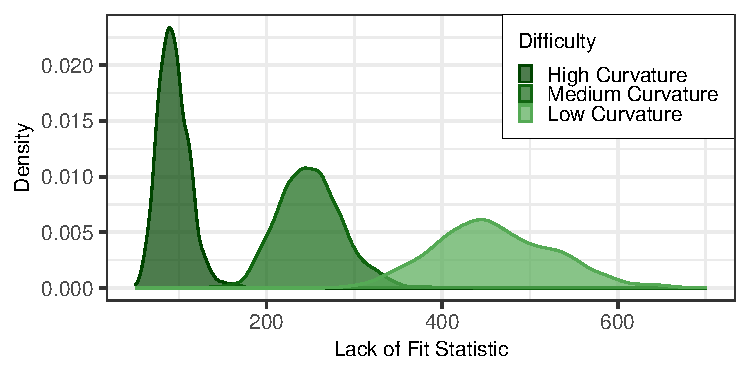
\includegraphics{index_files/figure-pdf/fig-lof-density-curves-1.pdf}

}

\caption{\label{fig-lof-density-curves}Density plot of the lack of fit
statistic showing separation of selected difficulty levels: High
(obvious curvature), Medium (noticeable curvature), and Low (almost
linear). Each density plot is the result of 1000 simulations from a
model \(y_i = \alpha\cdot e^{\beta\cdot x_i + \epsilon_i} + \theta\),
where \(\epsilon \sim N(0, \sigma^2)\). \(\alpha\) and \(\theta\) were
selected after manipulation of \(\beta\) and \(\sigma\) to ensure that
all data generated had similar \(y\) ranges so as not to provide visual
cues about model differences outside of the plot curvature.}

\end{figure}%

\subsection{Fine-Tuning Parameter
Choices}\label{fine-tuning-parameter-choices}

Once an appropriate set of parameters are identified using the numerical
screening method, it is important to calibrate these parameter
selections visually. No numerical statistic is a perfect measure of what
we actually see: at best, they are approximations of what we might
potentially see. We have found it to be useful to have one experimenter
calibrate the model parameters at a gross level, and then have another
experimenter narrow in on the parameters which are visually reasonable
within the selected range. Then, both examiners visually inspect a large
number of plots generated using those parameters to get a sense for how
difficult the task at hand is (this strategy is also described by Lu et
al. (Lu et al., 2022)). At some point, all experimenters become so
visually saturated with the nuances of the data generating mechanism
that it may become necessary to ``sanity check'' the protocol with
family members, friends, and colleagues. These informal surveys provide
extremely useful feedback and can help to counteract the visual
saturation of being immersed in the design of a visualization experiment
for months at a time.

\subsection{Visual Assessment is
Critical}\label{visual-assessment-is-critical}

We cannot overstate the importance of visual assessment of your model
stimuli, preferably with fresh eyes. We highly recommend performing
several rounds of think-aloud pilot testing before deploying an
experiment. In support of this assessment, we offer up a cautionary tale
of our own experience: that of (VanderPlas \& Hofmann, 2017), where we
designed an experiment to test which plot aesthetics promoted discovery
of linear trends and/or clusters.

The experiment was a full 2x3x3 factorial exploration of three data
generating parameters, with 3 replicates at each parameter combination
(54 data sets) and 10 aesthetic combinations (for a total of 540
lineups). Each lineup had 20 different sub-panels, so we should have
carefully visually inspected some 10,800 different panels. As is evident
from the fact that we're telling this story as a cautionary tale, we
missed a critical problem with our data-generating mechanism: when
clusters were assigned to randomly generated data after the fact, we
didn't control the cluster size, leading to clusters of one or two
points in relatively few sub-panels. This became particularly noticeable
when bounding ellipses were added to the plot, as the method used to
generate those ellipses required at least 3 points in the cluster. The
missing boundary ellipse in the corresponding sub-panels escaped our
notice during the stimuli proof-reading phase of the experiment, but did
not escape the notice of our participants, who only needed to examine
about 10 lineups each (around 200 panels). An example of one of the
problematic lineups is shown in Figure~\ref{fig-lineup-problems}: many
participants selected panel 16 because of the missing ellipse; not a
wrong choice, but certainly not the effect we intended to test.

\begin{figure}

\centering{

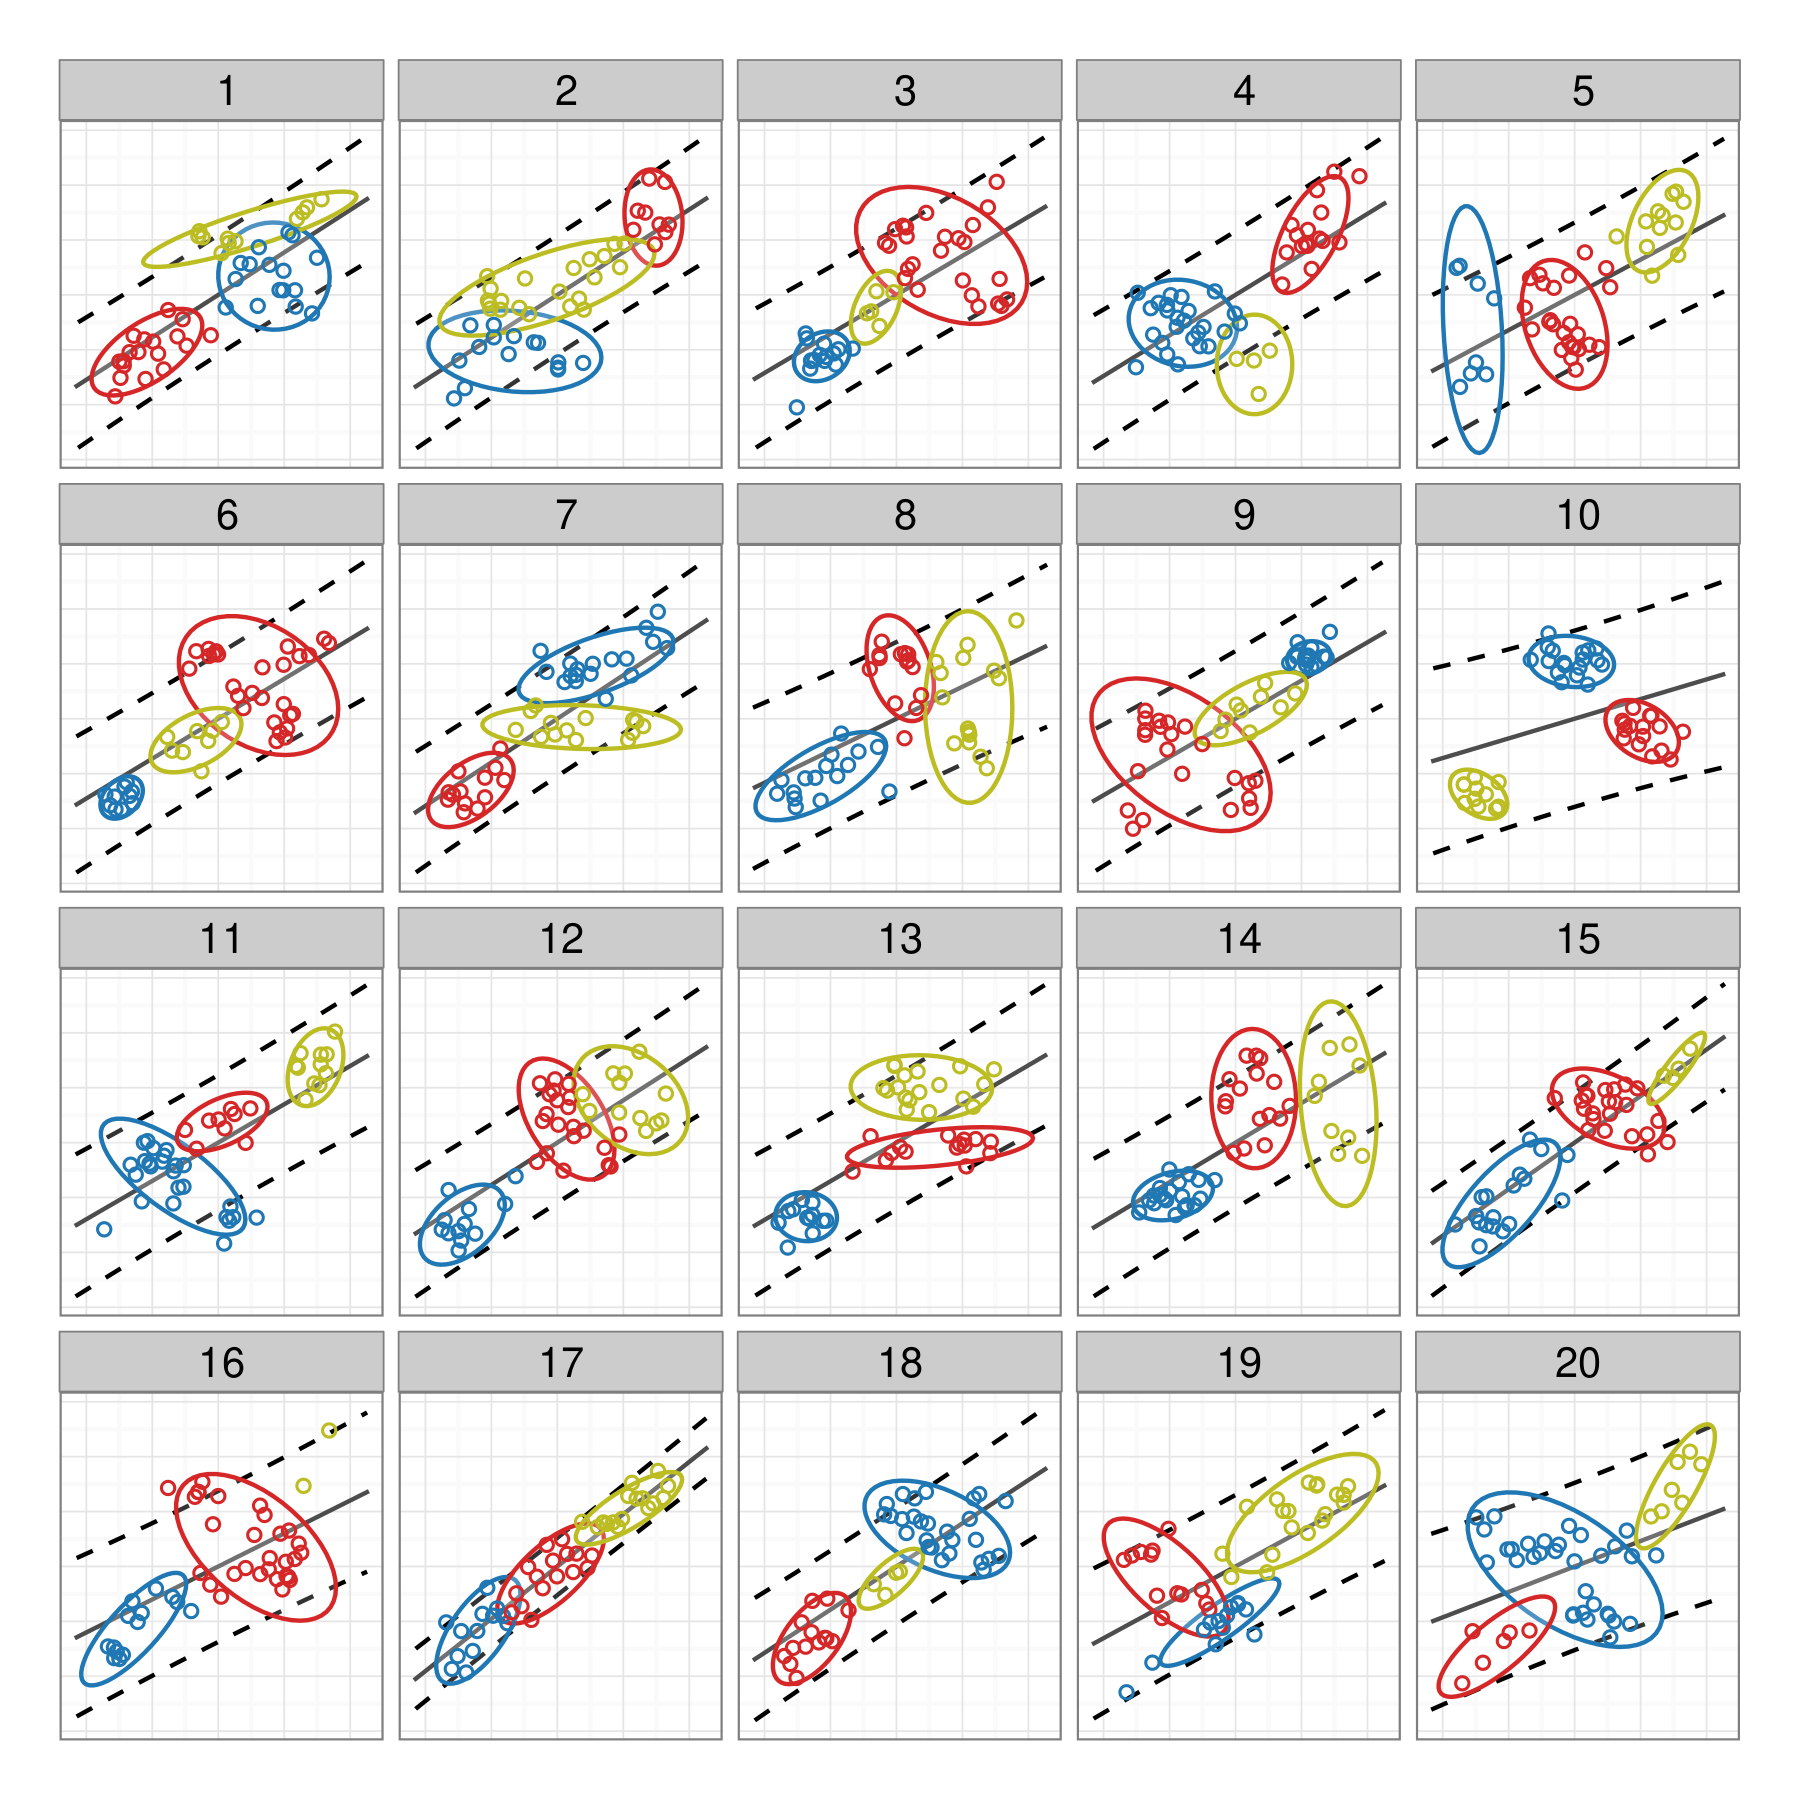
\includegraphics{lineup-missing-ellipse.png}

}

\caption{\label{fig-lineup-problems}A lineup from Vanderplas \& Hofmann
(VanderPlas \& Hofmann, 2017). Panel 10 shows the clustered target data
and panel 17 shows the target data with a strong linear relationship;
either of these target panels was the expected choice. Unfortunately,
panel 16 has only two bounding ellipses shown, which is an unintentional
difference that resulted from a faulty method for assigning clusters to
null plots; many participants selected this panel instead of one of the
target panels.}

\end{figure}%

One reason why it is so difficult to generate sampling models for visual
explorations is that our visual system is very, very good at finding
differences and unexpected results. We re-ran the experiment using a
different clustering method, and found that instead of noticing the
number of ellipses, when that variable was removed participants instead
cued in on the differences in size and shape of the ellipses formed
using k-means clustering after the data generating procedure. That is,
participants could still detect the artificial nature of the induced
clusters using other features. While it can be difficult to get the data
generating method right, it is essential to conducting visual
experiments that generalize well beyond the effects shown in a single
data set or phenomenon. The time and effort invested in this step at the
outset of the experiment pays dividends when it allows for clear
generalization of the experimental results to an entire statistical
concept rather than a single data set.

\section{Experimental Design Considerations}\label{sec-exp-design}

It would be difficult to develop a full data generating model without
some idea of the experimental design: the basic structure of the
parameters which are to be manipulated, how the users will be tested,
and so on. These experimental design factors are fairly natural for
scientists to accumulate over the course of imagining and planning an
experiment. When conducting graphical tests, however, there are
additional considerations beyond those taught in a standard experimental
design course.

The primary human design factor to be aware of is that visual tasks and
assessing statistical graphics can be extremely cognitively taxing. In
our experience, it is difficult to expect participants to evaluate more
than about 15 charts in one sitting. If users are asked to deeply engage
and answer multiple questions about each chart, this limit may be lower
(8-10), but even with a relatively simple task, as in lineup methods, it
is hard for participants to accurately evaluate more than about 15
charts. Tasks which are more interactive, such as `You Draw It', may be
somewhat easier for participants, but it is unlikely that participants
would be willing to complete more than about 20 tasks in one sitting
even with tasks that require fewer decisions and more engagement. At
some point, participants' interest in accuracy will decline, and the
researcher is better off using a larger number of participants
completing fewer tasks within the window where participants are
attentive and engaged.

It can be extremely helpful to include ``practice'' demonstrations of
the task to show the basic process, logic, and reasoning. While it is
tempting to make these tasks fully representative of the type of
judgement which will be required of participants, practice tasks which
are too close to the experimental task may bias participants; we have
found that it works well to have a relatively easy practice task which
utilizes a slightly different type of plot and/or type of data than what
will be tested in the experiment. In cases which require interactivity,
gif animations of the task being carried out are useful, as are
additional visual cues, such as the yellow box used in the `You Draw It'
task\footnote{See a gif of testing with `You Draw It'
  \href{https://i.imgur.com/GM5YSen.gif}{here}} to indicate that there
were points which were not completed.

While studies have found some relationship between lineup performance
and demographic factors (VanderPlas \& Hofmann, 2016), these differences
are relatively small when participants are recruited from online testing
platforms like Amazon Mechanical Turk or Prolific, or when participants
are recruited from a university student population. Studies have also
not found a strong relationship between visual task performance and
participant recruitment method (VanderPlas et al., 2019), perhaps in
part because demographics which use social media sites and demographics
completing online research tasks for pay overlap heavily. However, when
participants are recruited using a statistically representative sample
of the wider population, education becomes an extremely useful predictor
of ability to effectively read and draw conclusions about a chart (Rice
et al., 2024).\\
In almost every situation, though, we find that some participants are
very good at evaluating graphics and some participants are not; as a
result, it can be extremely helpful to use random effects models with an
effect for individual participants.

It may be useful to ask a few more demographic questions about STEM
education level for studies which ask more of participants from a
mathematical standpoint; while lineup studies have not found strong
associations with those variables, lineup studies also do not require
participants to engage with the data presented in a chart in a way that
requires higher-order mathematical reasoning. This has allowed us to
make the argument to IRB that our research is exempt, as we do not
collect enough demographic information to identify participants,
however, this has occasionally come at some cost. Our recent study
examining the use of log scales and exponential data was conducted using
Prolific, which recruits participants from around the world; we required
only that participants were fluent in English to participate. It was
only after the experiment was completed that we realized that different
countries introduce logarithms as a concept at different points during
primary and secondary education; it might be that individuals in some
countries have much more experience with log scales than those educated
in the United States. We mention this only to point out that while every
experiment contains a few missed opportunities, it is worth giving
careful thought to the demographic questions asked of participants and
what information may be helpful during the analysis stage.

In statistical design terms, most of our studies involve some type of
balanced incomplete block design, where participants are assigned to a
subset of experimental conditions which allow for estimation of the full
range of effects specified in the model. The particular structure of
these designs depends heavily on the factorial structure of the study,
but we typically arrange participants' trials to ensure that
participants see the same data set only once (where possible) and see as
many different experimental conditions as possible. It is also important
to reduce the impact of order effects using either e.g.~Latin square
designs or randomization where possible, but we recognize that this is
not always feasible due to the need to maintain participant naivete
during some portions of the experiment.

We have conducted visualization experiments using a wide variety of
tools: custom web servers running experiments using PHP black magic,
Qualtrics surveys for static graphics, and writing full Shiny
applications that control every part of the experimental process from
instructions to providing completion codes for payment. In our research,
Shiny has provided the right balance between control over the
experimental setting, procedure, etc. and the intricate details of web
server management, however, this balance is likely different for every
group and potentially for every experiment. Likewise, we have recruited
participants using Amazon Mechanical Turk, Prolific, Reddit and other
social media sites, and email; each recruitment method has trade-offs
between cost, convenience, and control over demographic variables. Rice
et al. (2024) recruited participants using NORC panel samples and found
that demographics in a fully representative sample are extremely
important. While using representative panel-based sampling methods is
considerably more expensive, there are generalizability concerns with
online recruitment methods such as Prolific and Mechanical Turk. People
who participate in studies via online platforms are more technologically
sophisticated and educated than the general population, and this bias
may significantly impact the conclusions.

\section{Pilot Testing and Quality Assurance}\label{sec-pilot-test}

Once the data generating model is set, the experiment is designed, and
the charts have been developed, the next step is an extensive round of
pilot testing. The goal of pilot testing is to ensure that the
experiment is set up properly and that no issues have been overlooked.
Pilot testing also provides an opportunity to ensure that directions are
clear, participants know what they are supposed to be doing, and to
estimate task completion time (which determines how much participant
will be paid on many online testing platforms). Our studies usually go
through 2-3 rounds of pilot testing, with at least one of those rounds
involving any relatives and friends who are less technologically savvy.
We also purposely include talented individuals who can accidentally
crash any testing applications. A final round of testing usually
includes any and all coworkers and friends who may be available for
10-15 minutes during the work day. Pilot study samples do not need to be
representative of any particular population, though we would caution
against using exclusively visualization researchers or statisticians in
your pilot sample because some issues are less likely to show up with
knowledgeable participants. In some studies, each participant may see a
new set of data, depending on how the study is designed. In these cases,
we highly recommend saving all generated data to a database as well, so
that it is possible to go back and examine exactly what happened and/or
how things went wrong. Hard drive space is extremely cheap relative to
almost any other cost in an experiment; saving all of the data is a
sensible measure.

One highly useful (but not strictly essential) component of an
experiment that can be set up during the pilot testing stage is a basic
analysis script which summarizes all data collected to date visually. We
have used such scripts in the past to produce automatically updating
dashboards or web pages, allowing for real time or near-real time
monitoring of data collection efforts. This provides an easy way to
summarize completion of the experiment so that individuals can receive
credit (if using services like MTurk or Prolific), but also allows
interested participants to see the data if recruiting participants who
are more likely to be interested in the results, as sometimes happens on
social media sites. As data collection online can also happen extremely
quickly (300 participants in \textless2h in our most recent Prolific
experiment), this can provide an illusion of control over the deluge of
data, allowing any issues to be spotted and resolved relatively quickly.
If server load is a potential issue, it may also help to release batches
of trials over a longer period of time in order to minimize the chance
of having to make participants wait for others to complete the task
before the server can handle additional connections\footnote{This is the
  one major drawback to our preferred solution of self-hosting a Shiny
  server to handle data collection: the free version of Shiny server is
  limited to about 15 connections at any given time. Prolific has
  recently added rate-limiting functions to the experimental control
  platform, which makes controlling the number of active jobs much
  easier.}.

\section{Analyzing the Data}\label{sec-analysis}

One constant with data analysis of these types of experiments is that no
matter how carefully the experiment is planned, designed, and executed,
there will be surprises. This is the dual curse and blessing of studying
human perception: the visual system never quite works the way that we
expect that it will, which provides endless fodder for science and
occasionally complicates the data analysis.

\subsection{Generalized Linear Mixed
Models}\label{generalized-linear-mixed-models}

The see-value approach (Chowdhury et al., 2020; Majumder et al., 2013;
VanderPlas et al., 2021) is extremely useful for single lineups, but
when a series of lineups that are part of a designed experiment are
used, generalized linear mixed models are a much simpler way to
summarize the overall effect of various manipulated factors (Hofmann et
al., 2012; Robinson, 2022; VanderPlas \& Hofmann, 2017). This approach
also works extremely well for psychometric experiments (VanderPlas \&
Hofmann, 2015), as psychometric models can be easily fit into the
framework of a generalized linear mixed model (Ju et al., 2024) that has
higher power than the Rasch models which were historically recommended
for these experiments. In addition, similar model structures can be used
to model accuracy, response time, and confidence, if all three types of
information are collected from participants during the experiment.

\subsection{Numerical Estimation}\label{numerical-estimation}

There are additional considerations that should be expected when asking
participants to estimate numerical quantities. Anchoring and rounding
cause participant responses to cluster in ways that can bias statistical
estimators, requiring methods designed for these types of data (Heitjan
\& Rubin, 1991; Tourangeau et al., 2000; Ushakov \& Ushakov, 2017). An
alternative approach is to analyze the data graphically using e.g.~a
combination of density and rug geoms for point estimates (as shown in
Figure~\ref{fig-density-rug}), or spaghetti plots for individual
response curves, with annotations to show anchor points. The advantage
of this approach is that it can accommodate extremely messy data without
requiring the extensive data cleaning and elimination of nonsensical
responses that might be necessary to fit a statistical model.

\begin{figure}

\centering{

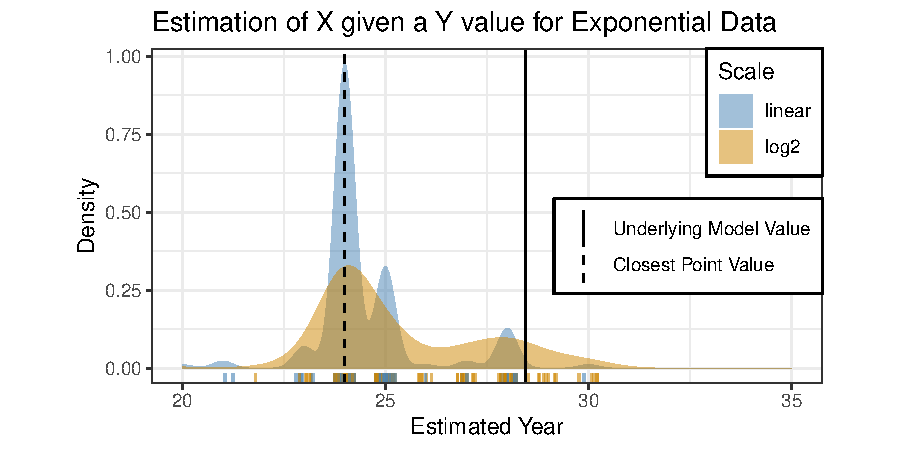
\includegraphics{index_files/figure-pdf/fig-density-rug-1.pdf}

}

\caption{\label{fig-density-rug}Density of participant estimates for the
year in which the population reaches 4000. Colors are associated to
scale - linear (blue) and log (orange) - and vertical lines indicate the
true value based on the underlying model equation (black solid) and
closest point value based on the simulated data set (black dashed). A
jittered rug plot along the \(x\)-axis shows where participant estimates
were made. The plot shows anchoring occurred to the closest point as
shown by an increase in density around the dashed line. Density peaks
occurred at whole values indicating rounding errors.}

\end{figure}%

\subsection{Direct Interactions}\label{direct-interactions}

If participants are making predictions and/or fitting visual statistics,
we have had success analyzing these responses by comparing the responses
to results from a statistical model to determine how visual statistics
differ from the numerical quantities derived mathematically. For
instance, we calculate the deviation between participant responses and
the linear regression in `You Draw It' experiments, then fitted
generalized additive mixed models to summarize the results across
different experimental conditions to assess how user-drawn predictions
deviated from the statistical estimates. In other direct interactions,
it may be useful to compare participant selections or annotations to
closest points on the chart to assess anchoring behavior; for discrete
selections, methods discussed in numerical estimation may also be
useful.

\subsection{Qualitative Responses}\label{qualitative-responses}

In many cases, it is helpful to combine participants' qualitative
reasoning with their quantitative responses to designed graphical
experiments. This approach provides useful context as to what
participants use to make their decisions, and can be useful when
assessing why unexpected responses occurred. We have used word clouds to
show overall themes in participant responses successfully in (VanderPlas
\& Hofmann, 2017); when paired with an appropriate linear model it
became clear that participants were fixating on unequal cluster size as
a visual cue. In cases where participants are provided with additional
utilities such as calculators and scratchpads, it can be useful to
select responses from individual participants which illustrate the
different types of calculations performed (but analyzing this data
quantitatively can be difficult).

\section{Conclusion}\label{conclusion}

Testing features of visualization graphically using online platforms
provides an incredibly powerful and efficient way to establish empirical
guidelines for statistical graphics and visualization. There are nearly
endless ways to combine web graphics, user interactions, and data
collection to get insight into perception and use of graphics in
practical settings. We have been continually surprised at the richness
of the data collected in these experiments and the ability to combine
qualitative and quantitative assessment to support conclusions that are
both nuanced and of practical use when deciding how to design and
present data using visualizations.

\section{References}\label{references}

\phantomsection\label{refs}
\begin{CSLReferences}{1}{0}
\bibitem[\citeproctext]{ref-allenVisualizingScientificData2016}
Allen, E. A., \& Erhardt, E. B. (2016). Visualizing {Scientific} {Data}.
In J. T. Cacioppo, L. G. Tassinary, \& G. G. Berntson (Eds.),
\emph{Handbook of {Psychophysiology}} (4th ed., pp. 679--697). Cambridge
University Press.
https://doi.org/\url{https://doi.org/10.1017/9781107415782.031}

\bibitem[\citeproctext]{ref-bertin1983semiology}
Bertin, J., \& Berg, W. J. (1983). \emph{Semiology of graphics:
Diagrams, networks, maps} (Vol. 1). University of Wisconsin press
Madison.

\bibitem[\citeproctext]{ref-d3}
Bostock, M., Ogievetsky, V., \& Heer, J. (2011). D³ {Data}-{Driven}
{Documents}. \emph{IEEE Transactions on Visualization and Computer
Graphics}, \emph{17}(12), 2301--2309.
https://doi.org/\url{https://doi.org/10/b7bhhf}

\bibitem[\citeproctext]{ref-bujaStatisticalInferenceExploratory2009}
Buja, A., Cook, D., Hofmann, H., Lawrence, M., Lee, E.-K., Swayne, D.
F., \& Wickham, H. (2009). Statistical inference for exploratory data
analysis and model diagnostics. \emph{Philosophical Transactions of the
Royal Society of London A: Mathematical, Physical and Engineering
Sciences}, \emph{367}(1906), 4361--4383.

\bibitem[\citeproctext]{ref-cairoFunctionalArtIntroduction2012}
Cairo, A. (2012). \emph{The {Functional} {Art}: {An} introduction to
information graphics and visualization}. New Riders.

\bibitem[\citeproctext]{ref-shiny}
Chang, W., Cheng, J., Allaire, J., Sievert, C., Schloerke, B., Xie, Y.,
Allen, J., McPherson, J., Dipert, A., \& Borges, B. (2021). \emph{Shiny:
Web application framework for r}.
\url{https://CRAN.R-project.org/package=shiny}

\bibitem[\citeproctext]{ref-chowdhury2018}
Chowdhury, N. R., Cook, D., Hofmann, H., \& Majumder, M. (2018).
Measuring Lineup Difficulty By Matching Distance Metrics With Subject
Choices in Crowd-Sourced Data. \emph{Journal of Computational and
Graphical Statistics}, \emph{27}(1), 132--145.
https://doi.org/\url{https://doi.org/10.1080/10618600.2017.1356323}

\bibitem[\citeproctext]{ref-niladriroychowdhurySeeValueApp2020}
Chowdhury, N. R., Diehl, H., Broderick, T., \& Stein, A. (2020).
\emph{The {See} {Value} {App}: {Visual} {Decision} {Making} for {Drug}
{Development}}. https://rinpharma.com/publication/rinpharma\_183/.

\bibitem[\citeproctext]{ref-clevelandShapeParameterTwoVariable1988}
Cleveland, W. S., McGill, M. E., \& McGill, R. (1988). The {Shape}
{Parameter} of a {Two}-{Variable} {Graph}. \emph{Journal of the American
Statistical Association}, \emph{83}(402), 289--300.
https://doi.org/\url{https://doi.org/10.1080/01621459.1988.10478598}

\bibitem[\citeproctext]{ref-clevelandGraphicalPerceptionGraphical1985}
Cleveland, W. S., \& McGill, R. (1985). Graphical {Perception} and
{Graphical} {Methods} for {Analyzing} {Scientific} {Data}.
\emph{Science}, \emph{229}(4716), 828--833.
https://doi.org/\url{https://doi.org/10.1126/science.229.4716.828}

\bibitem[\citeproctext]{ref-cookFoundationAvailableThinking2021}
Cook, D., Reid, N., \& Tanaka, E. (2021). The {Foundation} {Is}
{Available} for {Thinking} {About} {Data} {Visualization}
{Inferentially}. \emph{Harvard Data Science Review}, \emph{3}(3).
https://doi.org/\url{https://doi.org/10.1162/99608f92.8453435d}

\bibitem[\citeproctext]{ref-croxtonGraphicComparisonsBars1932}
Croxton, F. E. (1932). Graphic {Comparisons} by {Bars}, {Squares},
{Circles}, and {Cubes}. \emph{Journal of the American Statistical
Association}, \emph{27}(177), 54--60.

\bibitem[\citeproctext]{ref-croxtonBarChartsCircle1927}
Croxton, F. E., \& Stryker, R. E. (1927). Bar {Charts} {Versus} {Circle}
{Diagrams}. \emph{Journal of the American Statistical Association},
\emph{22}(160), 473--482.
https://doi.org/\url{https://doi.org/10.2307/2276829}

\bibitem[\citeproctext]{ref-curcio1987comprehension}
Curcio, F. (1987). Comprehension of mathematical relationships expressed
in graphs. \emph{Journal for Research in Mathematics Education},
\emph{18}(5), 382--393.

\bibitem[\citeproctext]{ref-desnoyersTaxonomyVisualsScience2011}
Desnoyers, L. (2011). \emph{Toward a {Taxonomy} of {Visuals} in
{Science} {Communication}}. \emph{58}(2), 16.

\bibitem[\citeproctext]{ref-dunbar1995scientists}
Dunbar, K. (1995). How scientists really reason: {Scientific} reasoning
in real-world laboratories. \emph{The Nature of Insight}, \emph{18},
365--395.

\bibitem[\citeproctext]{ref-eellsRelativeMeritsCircles1926}
Eells, W. C. (1926). The {Relative} {Merits} of {Circles} and {Bars} for
{Representing} {Component} {Parts}. \emph{Journal of the American
Statistical Association}, \emph{21}(154), 119--132.
https://doi.org/\url{https://doi.org/10.2307/2277140}

\bibitem[\citeproctext]{ref-fewInformationDashboardDesign2006}
Few, S. (2006). \emph{Information {Dashboard} {Design}: {The}
{Effective} {Visual} {Communication} of {Data}}. O'Reilly Media,
Incorporated.

\bibitem[\citeproctext]{ref-friel2001making}
Friel, S., Curcio, F., \& Bright, G. (2001). Making sense of graphs:
Critical factors influencing comprehension and instructional
implications. \emph{Journal for Research in Mathematics Education},
\emph{32}(2), 124--158.

\bibitem[\citeproctext]{ref-glazer2011challenges}
Glazer, N. (2011). Challenges with graph interpretation: A review of the
literature. \emph{Studies in Science Education}, \emph{47}(2), 183--210.

\bibitem[\citeproctext]{ref-haemerDoubleScalesAre1948}
Haemer, K. W. (1948). Double {Scales} are {Dangerous}. \emph{The
American Statistician}, \emph{2}(3), 24--24.
https://doi.org/\url{https://doi.org/10.1080/00031305.1948.10501588}

\bibitem[\citeproctext]{ref-heitjanIgnorabilityCoarseData1991}
Heitjan, D. F., \& Rubin, D. B. (1991). Ignorability and {Coarse}
{Data}. \emph{The Annals of Statistics}, \emph{19}(4), 2244--2253.
https://doi.org/\url{https://doi.org/10.1214/aos/1176348396}

\bibitem[\citeproctext]{ref-power}
Hofmann, H., Follett, L., Majumder, M., \& Cook, D. (2012). Graphical
tests for power comparison of competing designs. \emph{IEEE Transactions
on Visualization and Computer Graphics}, \emph{18}(12), 2441--2448.
\url{https://doi.org/f4fwkz}

\bibitem[\citeproctext]{ref-vonhuhnFurtherStudiesGraphic1927}
Huhn, R. von. (1927). Further {Studies} in the {Graphic} {Use} of
{Circles} and {Bars}: {A} {Discussion} of the {Eell}'s {Experiment}.
\emph{Journal of the American Statistical Association}, \emph{22}(157),
31--39. https://doi.org/\url{https://doi.org/10.2307/2277346}

\bibitem[\citeproctext]{ref-hullmanDesigningInteractiveExploratory2021}
Hullman, J., \& Gelman, A. (2021). Designing for {Interactive}
{Exploratory} {Data} {Analysis} {Requires} {Theories} of {Graphical}
{Inference}. \emph{Harvard Data Science Review}, \emph{3}(3).
https://doi.org/\url{https://doi.org/10.1162/99608f92.3ab8a587}

\bibitem[\citeproctext]{ref-asme-standards-graphics}
Joint committee on standards for graphic presentation. (1915).
\emph{Publications of the American Statistical Association},
\emph{14}(112), 790--797. \url{http://www.jstor.org/stable/2965153}

\bibitem[\citeproctext]{ref-juOneModelThat2024}
Ju, W. (Will)., Vanderplas, S., \& Hofmann, H. (2024). One {Model} that
fits them {All}: {Psychometrics} with {Generalized Linear Mixed Effects
Models}. \emph{Electronic Imaging}, 1--9.
\url{https://doi.org/10.2352/EI.2023.35.1.VDA-A01}

\bibitem[\citeproctext]{ref-katzYouDrawIt2017}
Katz, J. (2017). You {Draw} {It}: {Just} {How} {Bad} {Is} the {Drug}
{Overdose} {Epidemic}? \emph{The New York Times}.
\url{https://www.nytimes.com/interactive/2017/04/14/upshot/drug-overdose-epidemic-you-draw-it.html}

\bibitem[\citeproctext]{ref-kirschenbaum2003comparative}
Kirschenbaum, S. S. (2003). Comparative {Cognitive} {Task} {Analysis}:
{The} {Cognition} of {Weather} {Forecasting}. \emph{Proceedings of the
{Human} {Factors} and {Ergonomics} {Society} {Annual} {Meeting}},
\emph{47}, 473--477.
https://doi.org/\url{https://doi.org/10.1177/154193120304700347}

\bibitem[\citeproctext]{ref-kosslynGraphDesignEye2006}
Kosslyn, S. M. (2006). \emph{Graph {Design} for the {Eye} and {Mind}}.
Oxford University Press.

\bibitem[\citeproctext]{ref-loyDiagnosticToolsHierarchical2013}
Loy, A., \& Hofmann, H. (2013). Diagnostic tools for hierarchical linear
models. \emph{Wiley Interdisciplinary Reviews: Computational
Statistics}, \emph{5}(1), 48--61.
https://doi.org/\url{https://doi.org/10.1002/wics.1238}

\bibitem[\citeproctext]{ref-luModelingJustNoticeable2022}
Lu, M., Lanir, J., Wang, C., Yao, Y., Zhang, W., Deussen, O., \& Huang,
H. (2022). Modeling {Just} {Noticeable} {Differences} in {Charts}.
\emph{IEEE Transactions on Visualization and Computer Graphics},
\emph{28}(1), 718--726.
https://doi.org/\url{https://doi.org/10.1109/TVCG.2021.3114874}

\bibitem[\citeproctext]{ref-majumderValidationVisualStatistical2013}
Majumder, M., Hofmann, H., \& Cook, D. (2013). Validation of visual
statistical inference, applied to linear models. \emph{Journal of the
American Statistical Association}, \emph{108}(503), 942--956.
https://doi.org/\url{https://doi.org/10/f5gntt}

\bibitem[\citeproctext]{ref-R}
R Core Team. (2022). \emph{R: A language and environment for statistical
computing}. R Foundation for Statistical Computing.
\url{https://www.R-project.org/}

\bibitem[\citeproctext]{ref-ribeccaSearchChartsData}
Ribecca, S. (2022). \emph{The data visualisation catalogue}.
https://datavizcatalogue.com.

\bibitem[\citeproctext]{ref-riceTestingPerceptualAccuracy2024}
Rice, K., Hofmann, H., du Toit, N., \& Mulrow, E. (2024). Testing
{Perceptual Accuracy} in a {U}.{S}. {General Population Survey Using
Stacked Bar Charts}. \emph{Journal of Data Science}, 1--18.
\url{https://doi.org/10.6339/24-JDS1121}

\bibitem[\citeproctext]{ref-emily-diss}
Robinson, E. A. (2022). \emph{Human {Perception} of {Exponentially}
{Increasing} {Data} {Displayed} on a {Log} {Scale} {Evaluated} {Through}
{Experimental} {Graphics} {Tasks}} {[}Doctoral, University of Nebraska,
Lincoln{]}.
\url{https://github.com/earobinson95/EmilyARobinson-UNL-dissertation/raw/main/EmilyRobinson-final-dissertation.pdf}

\bibitem[\citeproctext]{ref-tourangeau_rips_rasinski_2000}
Tourangeau, R., Rips, L. J., \& Rasinski, K. (2000). \emph{The
psychology of survey response}. Cambridge University Press.
https://doi.org/\url{https://doi.org/10.1017/CBO9780511819322}

\bibitem[\citeproctext]{ref-traftonTurningPicturesNumbers2000}
Trafton, G. J., Kirschenbaum, S. S., Tsui, T. L., Miyamoto, R. T.,
Ballas, J. A., \& Raymond, P. D. (2000). Turning pictures into numbers:
Extracting and generating information from complex visualizations.
\emph{International Journal of Human-Computer Studies}, \emph{53}(5),
827--850. \url{https://doi.org/10.1006/ijhc.2000.0419}

\bibitem[\citeproctext]{ref-tufte}
Tufte, E. (1991). \emph{The {Visual} {Display} of {Quantitative}
{Information}} (2nd ed.). Graphics Press.

\bibitem[\citeproctext]{ref-ushakovStatisticalAnalysisRounded2017}
Ushakov, N. G., \& Ushakov, V. G. (2017). Statistical analysis of
rounded data: {Recovering} of information lost due to rounding.
\emph{Journal of the Korean Statistical Society}, \emph{46}(3),
426--437.
https://doi.org/\url{https://doi.org/10.1016/j.jkss.2017.01.003}

\bibitem[\citeproctext]{ref-vanderplasDesigningGraphicsRequires2021}
VanderPlas, S. (2021). Designing {Graphics} {Requires} {Useful}
{Experimental} {Testing} {Frameworks} and {Graphics} {Derived} {From}
{Empirical} {Results}. \emph{Harvard Data Science Review}, \emph{3}(3).
https://doi.org/\url{https://doi.org/10.1162/99608f92.7d099fd0}

\bibitem[\citeproctext]{ref-vanderplasEscapingFlatlandGraphics2024}
Vanderplas, S., Blankenship, E., \& Wiederich, T. (2024). Escaping
{Flatland}: {Graphics}, {Dimensionality}, and~{Human Perception}. In H.
Mori \& Y. Asahi (Eds.), \emph{Human {Interface} and the {Management} of
{Information}} (pp. 140--156). Springer Nature Switzerland.
\url{https://doi.org/10.1007/978-3-031-60114-9_11}

\bibitem[\citeproctext]{ref-vanderplasTestingStatisticalCharts2020}
Vanderplas, S., Cook, D., \& Hofmann, H. (2020). Testing {Statistical}
{Charts}: {What} {Makes} a {Good} {Graph}? \emph{Annual Review of
Statistics and Its Application}, \emph{7}(1).
https://doi.org/\url{https://doi.org/10.1146/annurev-statistics-031219-041252}

\bibitem[\citeproctext]{ref-vanderplasFramedReproducingRevisiting2019}
VanderPlas, S., Goluch, R., \& Hofmann, H. (2019). Framed! {Reproducing}
and {Revisiting} 150 year old charts. \emph{Journal of Computational and
Graphical Statistics}.
https://doi.org/\url{https://doi.org/10.1080/10618600.2018.1562937}

\bibitem[\citeproctext]{ref-sineillusion}
VanderPlas, S., \& Hofmann, H. (2015). Signs of the {Sine}
{Illusion}---{Why} {We} {Need} to {Care}. \emph{Journal of Computational
and Graphical Statistics}, \emph{24}(4), 1170--1190.
https://doi.org/\url{https://doi.org/10.1080/10618600.2014.951547}

\bibitem[\citeproctext]{ref-vanderplasSpatialReasoningData2016a}
VanderPlas, S., \& Hofmann, H. (2016). Spatial {Reasoning} and {Data}
{Displays}. \emph{IEEE Transactions on Visualization and Computer
Graphics}, \emph{22}(1), 459--468.
https://doi.org/\url{https://doi.org/10.1109/TVCG.2015.2469125}

\bibitem[\citeproctext]{ref-clusters}
VanderPlas, S., \& Hofmann, H. (2017). Clusters {Beat} {Trend}!?
{Testing} {Feature} {Hierarchy} in {Statistical} {Graphics}.
\emph{Journal of Computational and Graphical Statistics}, \emph{26}(2),
231--242. \url{https://doi.org/10.1080/10618600.2016.1209116}

\bibitem[\citeproctext]{ref-vanderplasStatisticalSignificanceCalculations2021}
VanderPlas, S., Röttger, C., Cook, D., \& Hofmann, H. (2021).
Statistical significance calculations for scenarios in visual inference.
\emph{Stat}, \emph{10}(1).
https://doi.org/\url{https://doi.org/10.1002/sta4.337}

\bibitem[\citeproctext]{ref-ggplot2}
Wickham, H. (2016). \emph{ggplot2: Elegant graphics for data analysis}.
Springer-Verlag New York. \url{https://ggplot2.tidyverse.org}

\bibitem[\citeproctext]{ref-wickhamGraphicalInferenceInfovis2010}
Wickham, H., Cook, D., Hofmann, H., \& Buja, A. (2010). Graphical
inference for infovis. \emph{IEEE Transactions on Visualization and
Computer Graphics}, \emph{16}(6), 973--979.
https://doi.org/\url{https://doi.org/10.1109/TVCG.2010.161}

\bibitem[\citeproctext]{ref-wilkinsonGrammarGraphics1999}
Wilkinson, L. (1999). \emph{The grammar of graphics}. Springer.
\url{http://public.ebookcentral.proquest.com/choice/publicfullrecord.aspx?p=3085765}

\bibitem[\citeproctext]{ref-wood1968objectives}
Wood, R. (1968). Objectives in the teaching of mathematics.
\emph{Educational Research}, \emph{10}(2), 83--98.

\end{CSLReferences}




\end{document}
